\section{Theory}
\markright{Theory}

The transformation of an AC signal into a DC signal is fundamentally achieved through the process of
rectification. This process relies on the inherent characteristic curve of diodes, which only permit
current to flow when they are in a forward-biased condition and act as an open circuit when
reverse-biased \cite{lab04_mehta2012}. When an alternating voltage is applied across a diode, it will
only permit the conduction of the positive half-cycle—depending on the specific orientation of the
diode—while cutting off the opposite half-cycle during its reverse-bias state \cite
{lab04_boylestad2013}. Consequently, the load obtains a unidirectional DC signal. Diode rectifiers are
primarily classified into two types: the half-wave rectifier and the full-wave rectifier \cite
{lab04_mehta2012}.

In a full-wave rectifier circuit, both half-cycles of the input AC signal are utilized and present in
the output, offering significantly higher efficiency than half-wave designs \cite{lab04_boylestad2013}.
Two primary circuit configurations are utilized as full-wave rectifiers: the center-tapped transformer
rectifier and the bridge rectifier \cite{lab04_mehta2012}. The center-tapped transformer design links
the transformer ends to two diodes, with the load situated between the diode junction and the center
tap of the secondary winding \cite{lab04_boylestad2013}. The circuit diagram and the resulting wave
shapes for this configuration are illustrated in Figure \ref{lab04_fig:center_tapped}.

\begin{figure}[H]
  \centering
  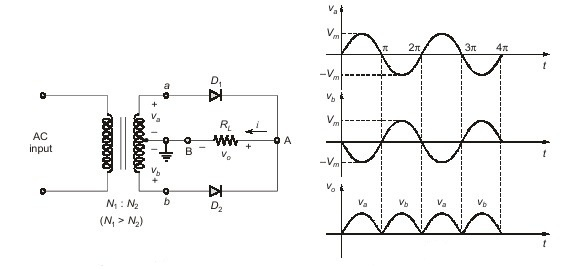
\includegraphics[width=0.6\textwidth]{lab-04/assets/theory-center-tapped.jpg}
  \caption{Full wave rectifier using center tapped transformer showing input and output waveforms. \cite{lab04_madeeasy_rectifier}}
  \label{lab04_fig:center_tapped}
\end{figure}

Compared to the half-wave alternative, the center-tapped circuit offers several distinct advantages,
including a higher average DC output and reduced power waste \cite{lab04_mehta2012}. Additionally, the
output waveform produced by this method is notably smoother than that of a half-wave rectifier \cite
{lab04_boylestad2013}. However, this configuration also presents specific drawbacks, as it demands
additional physical room within a chassis and is often considered sturdy or bulky due to the
requirements of the specialized center-tapped transformer \cite{lab04_mehta2012}.

The full-wave bridge rectifier is a circuit that converts both half-cycles of an input alternating
current (AC) to direct current (DC) using four diodes arranged in a bridge pattern \cite
{lab04_boylestad2013}. This design is highly advantageous because it mitigates the drawbacks associated
with the center-tapped transformer, specifically eliminating the need for a specialized tap while
maintaining high efficiency \cite{lab04_mehta2012}. The standard bridge configuration is shown in
Figure \ref{lab04_fig:bridge_rectifier}.

\begin{figure}[htbp]
  \centering

  \begin{subfigure}{0.40\textwidth}
    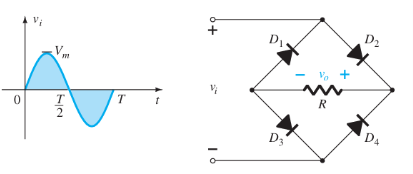
\includegraphics{lab-04/assets/theory-full-wave-bridge-rectifier.png}
    \caption{}
  \end{subfigure}
  \begin{subfigure}{0.30\textwidth}
    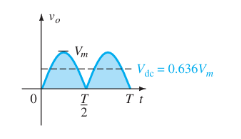
\includegraphics{lab-04/assets/theory-full-wave-resulting-wave.png}
    \caption{}
  \end{subfigure}

  \caption{Full Wave Bridge Rectifier (a) circuit and (b) resulting wave shapes.\cite{lab04_boylestad2013}}
  \label{lab04_fig:bridge_rectifier}
\end{figure}

On the other hand, even a full-wave rectifier is unable to provide a perfectly steady DC voltage on its
own; the output is typically rippled as a result of the pulsating nature of the rectified sine wave
\cite{lab04_mehta2012}. To achieve a more stable output, a filter capacitor is placed across the load,
allowing this ripple to be significantly lessened by smoothing the voltage fluctuations \cite
{lab04_boylestad2013}. The circuit implementation for a bridge rectifier utilizing a capacitor filter
is shown in Figure \ref{lab04_fig:bridge_capacitor}.

\begin{figure}[H]
  \centering
  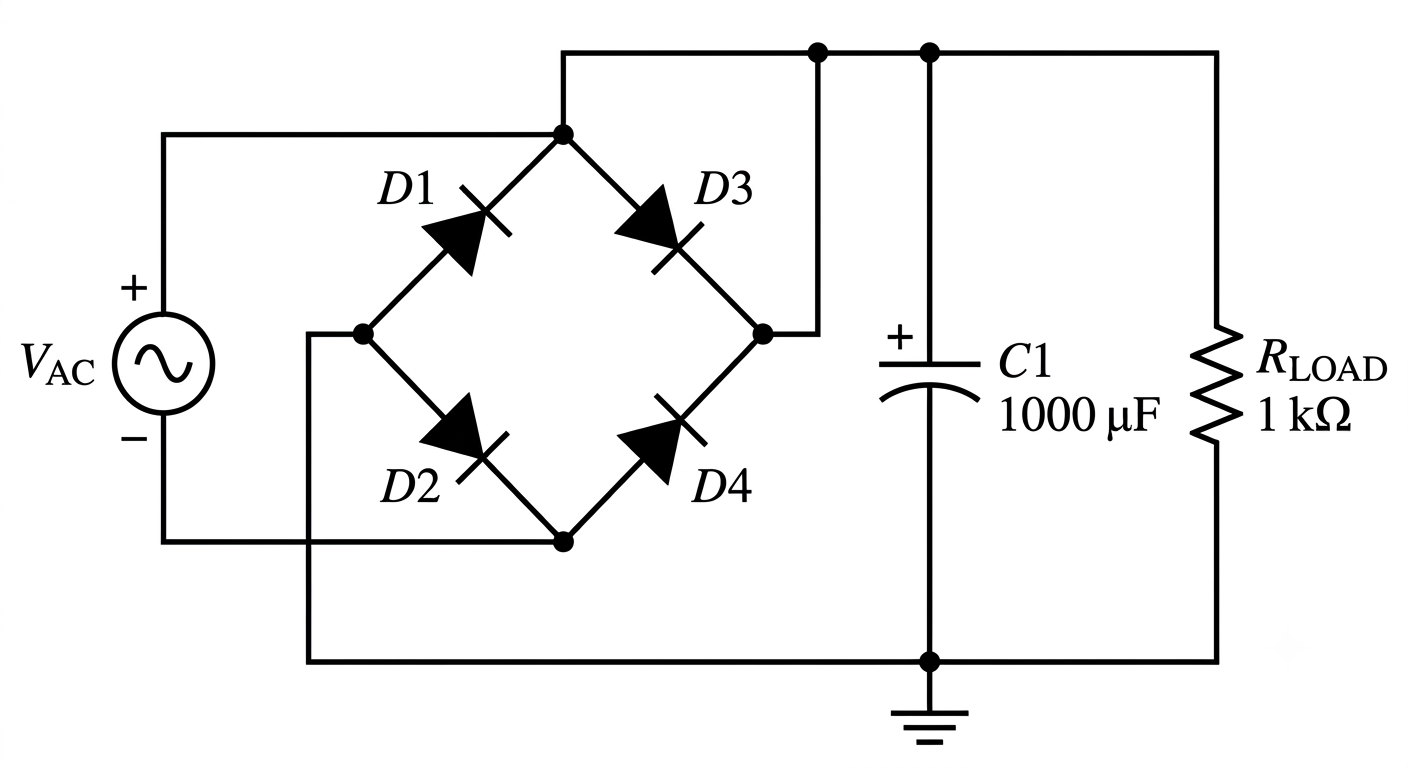
\includegraphics[width=0.8\textwidth]{lab-04/assets/theory-full-wave-bridge-rectifier-with-filter.png}
  \caption{Circuit Diagram for Full Wave Bridge Rectifier including a filter capacitor. \cite
    {lab04_gemini_bridge_filter_circuit}}
  \label{lab04_fig:bridge_capacitor}
\end{figure}
